\documentclass[11pt,a4paper]{article}
\usepackage[margin=2.3cm]{geometry}
\usepackage{booktabs}
\usepackage{graphicx}
\usepackage{caption}
\usepackage{amsmath}
\usepackage{microtype}
\usepackage{xcolor}
\usepackage[colorlinks=true,linkcolor=blue!60!black,urlcolor=blue!60!black]{hyperref}
\captionsetup{font=small,labelfont=bf}
\graphicspath{{plots/}}
\newcommand{\ntasks}{7,381}
\newcommand{\nholes}{2,319,574}
\newcommand{\nholesteps}{4,500,561}
\newcommand{\njustshare}{99.5}
\newcommand{\nprovedshare}{99.8}
\newcommand{\nkept}{11,980}
\newcommand{\nskipped}{543}
\newcommand{\nfully}{4,496}
\newcommand{\nvalid}{1,506}
\newcommand{\nuntagged}{3,358}
\newcommand{\nfullyclean}{1,822}
\newcommand{\nfullycleanholey}{316}
\newcommand{\npivot}{206}
\newcommand{\nhoistto}{8}
\newcommand{\nrecheckto}{24}
\newcommand{\eggshare}{35}
\newcommand{\nclosednorm}{694,786}
\newcommand{\normshare}{30.0}
\newcommand{\passhours}{139}
\newcommand{\cpuhours}{1,217}
\newcommand{\wallhours}{152}

\emergencystretch=2em

\newcommand{\UF}{QF\_UF}
\newcommand{\LIA}{QF\_LIA}
\newcommand{\LRA}{QF\_LRA}
\newcommand{\code}[1]{\texttt{#1}}

\title{Justifying cvc5 rewrite holes with egglog and RARE:\\
  run \code{rw2} on \UF{}, \LIA{} and \LRA{}, and the state of the tooling}
\author{Carcara branch \code{egglog/rewrite-holes}}
\date{Run of 2026-09-24/25 (binary \code{3f982c71}) -- report of 2026-09-25 (tooling at \code{fedf0b31})}

\begin{document}
\maketitle

\begin{abstract}
  cvc5's Alethe proofs leave the rewrites its post-processor cannot expand
  as premise-free \code{hole} steps tagged \code{MACRO\_REWRITE} or
  \code{MACRO\_SR\_PRED\_INTRO}. Carcara's hole pipeline hoists and prunes
  the repeated ones, tries each with a checker-certified normalizer and,
  where that does not close it, with egglog saturation over a RARE rule
  set, reconstructs an Alethe subproof from the saturated e-graph, and
  re-checks the result. This report summarises one run over \ntasks{}
  benchmarks of \UF{}, \LIA{} and \LRA{}, every one with a complete cvc5
  proof (\nholesteps{} hole steps, \nholes{} distinct holes after hoist and
  prune). Of the holes attempted, \njustshare\% are justified with Alethe
  steps and \nprovedshare\% are proved (justified, or proved by egglog and
  lost in the reconstruction); the normalizer alone settles \normshare\%
  of them before egglog runs. \nfully{} proofs come out with every hole
  justified and \nvalid{} re-check \code{valid}; the gap between the two is
  the \nuntagged{} proofs that carry a hole the pipeline never attempts
  (cvc5's untagged arithmetic and subtype-elimination trust steps), plus
  \nfullycleanholey{} proofs in which a certificate itself falls back to a
  trust step. The per-proof budget, which dominated the previous run, binds
  \nskipped{} holes. The \nkept{} kept holes are: \eggshare\% egglog time
  or memory kills, two thirds of them in four \LRA{} families; a third the
  reconstruction's own losses on \UF{}'s coarse Boolean holes (no
  certificate, or the search killed after egglog had proved the goal);
  and a small honest residue of goals outside the rule set. The
  reconstruction and elaboration causes were reproduced after the run and
  are fixed at \code{fedf0b31}; what remains is arithmetic, and the last
  section plans it.
\end{abstract}

\section{Setup}

\paragraph{Pipeline.} Each benchmark runs through the runner
\code{run-holes-rw2.sh} on one 8-core slot:
\begin{enumerate}
  \item cvc5 (branch \code{alethe-rewrite-granularity}, static
    \code{bin/cvc5-rw}) solves and prints an Alethe proof with the options\\
    \code{--proof-granularity=rewrite --proof-alethe-res-pivots}\\
    \code{--proof-elim-subtypes --print-arith-lit-token}.\\
    A rewrite the post-processor cannot expand is printed as
    \code{(step t (cl (= t t')) :rule hole :args ("MACRO\_REWRITE"
    "RW\_REWRITE"))} (or \code{"MACRO\_SR\_PRED\_INTRO"}), premise-free.
    A step it neither expands nor tags stays an \emph{untagged} hole the
    pipeline does not attempt: \code{THEORY\_INFERENCE\_ARITH},
    \code{MACRO\_THEORY\_REWRITE\_RCONS\_SIMPLE}, the
    \code{TRUST\_THEORY\_REWRITE} of subtype elimination, \code{DIAMONDS}.
  \item \textbf{Hoist + prune}: \code{carcara elaborate --pipeline hoist
    prune}. Repeated hole subproofs are lifted to the top level
    (\code{ho*} steps) and duplicates dropped; this is where \LIA{}'s
    1.97\,M hole steps become 748\,k distinct holes and \LRA{}'s 1.24\,M
    become 505\,k (\UF{} loses 5\%).
  \item \textbf{Elaboration pass}: \code{carcara elaborate --pipeline hole
    --elaborate-hole-rewrites} with eight isolated workers (one child
    process per hole), smallest goal first, the set-form list encoding,
    the normalizer prepass, sort guards and shared-subterm abstraction at
    16 nodes. A hole is \emph{justified} when a certificate is extracted
    from the saturated e-graph, verified by an independent rule checker,
    and emitted as Alethe steps; otherwise it is \emph{kept} with the
    worker's reason, or \emph{skipped} when the pass budget ran out first.
  \item \textbf{Re-check} of the elaborated proof by \code{carcara check}
    with the RARE file, so that \code{rare\_rewrite} steps check.
\end{enumerate}
There is no separate checking pass. ``Proved'' is derived from the
elaboration pass as justified + no certificate + checker rejected + killed
after egglog: a hole whose worker died in the serialization or the search
had its goal proved by egglog. The derivation is conservative in one
direction only -- check and reconstruction share the 60\,s, so a goal a
pure checking pass would have proved but that was killed \emph{inside}
egglog here counts as lost. The pass uses the RARE file
\code{holes-rw2.rare}, 171 rules: cvc5's \code{big.rare} of the time,
including its 80 bit-vector and string rules, plus \code{ite-eq},
\code{distinct-false} and the eight Boolean absorption, flattening and
duplicate rules over \code{:list} parameters. (The local file was trimmed
to 91 rules after the upload, on 2026-09-24; the cluster's copy, checked
by checksum, is the 171-rule one, so every number here is with the
larger file. The trimmed file roughly halves the fixed cost of a hole in
local measurements.) Carcara is the static build of commit
\code{3f982c71}.

\paragraph{Limits.} Per-hole limits are hard kills of the worker; the
pass budget is a deadline counted from the CLI's start, after which the
remaining holes are \emph{skipped} and the proof is emitted with what was
achieved.
\begin{center}\small
\begin{tabular}{ll}
\toprule
stage & limit \\
\midrule
cvc5 solve + proof & 60 s (\code{--tlimit}), external kill at 75 s \\
hoist + prune & 300 s (the proof is then checked as it stands) \\
elaboration pass & 1,500 s per proof; 60 s and 6 GB per hole; external kill at 1,600 s \\
\quad egglog & growth caps 120\,M (arithmetic) / 20\,M tuples, memory soft cap 5.4 GB \\
re-check of the elaborated proof & 900 s \\
SLURM job & partition \code{octa}, 8 cpus, 60 GB, 3,100 s wall, two tasks per node \\
\bottomrule
\end{tabular}
\end{center}

\paragraph{Benchmarks.} The sets \code{rw\_QF\_UF} (4,316), \code{rw\_QF\_LIA}
(2,541) and \code{rw\_QF\_LRA} (524): the benchmarks cvc5 proved within 60\,s
in the previous run of the pipeline (\code{rw1}, 2026-09-22/23), so no task
is spent on a solver time-out and every proof is complete. The run took
\wallhours{} task-hours on two tasks per node, about \cpuhours{} core-hours
reserved; the elaboration passes themselves sum to \passhours{} hours.

\section{Yield}

Table~\ref{tab:yield} gives the yield per logic; Figure~\ref{fig:sizes}
the distribution of holes per proof after hoist and prune. \UF{} proofs are
uniform (p50 253 holes, max 2k); \LIA{} has a fifth of its proofs with at
most a dozen holes and a tail to 9k; \LRA{}'s tail reaches 15k, six proofs
holding a fifth of the logic's holes.

\begin{table}[htbp]\centering\small
\resizebox{\textwidth}{!}{\begin{tabular}{lrrrrrrrr}
\toprule
logic & proofs & hole steps & holes & p50 & p90 & max & every hole justified & re-check \texttt{valid} \\
\midrule
QF\_UF & 4,316 & 1,288,303 & 1,221,095 & 253 & 469 & 2,062 & 1,907 (44.2\%) & 322 \\
QF\_LIA & 2,541 & 1,973,773 & 747,899 & 15 & 643 & 8,763 & 2,263 (89.1\%) & 982 \\
QF\_LRA & 524 & 1,238,485 & 504,702 & 64 & 2,662 & 15,544 & 326 (62.2\%) & 202 \\
\bottomrule
\end{tabular}
}
\caption{Yield. ``hole steps'' are the \code{hole} steps in cvc5's proof,
  ``holes'' the distinct goals left after hoist and prune, with the median
  (p50), 90th percentile and maximum per proof. ``every hole justified''
  counts the proofs in which no attempted hole was kept or skipped, with
  the share of the logic's proofs; ``re-check \code{valid}'' the proofs
  whose elaborated output passed the final check with no \code{hole} step
  at all.}\label{tab:yield}
\end{table}

\begin{figure}[htbp]\centering
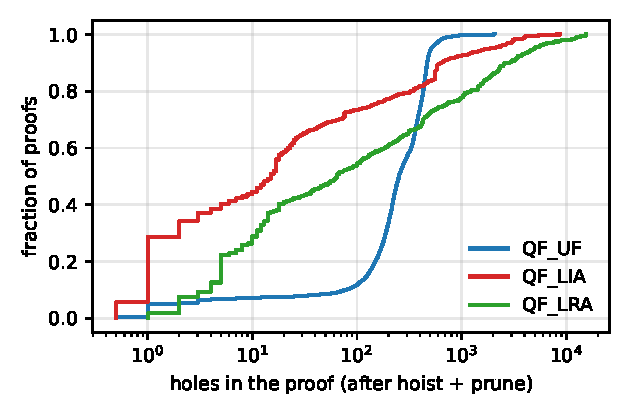
\includegraphics[width=.48\textwidth]{holes-per-proof}\hfill
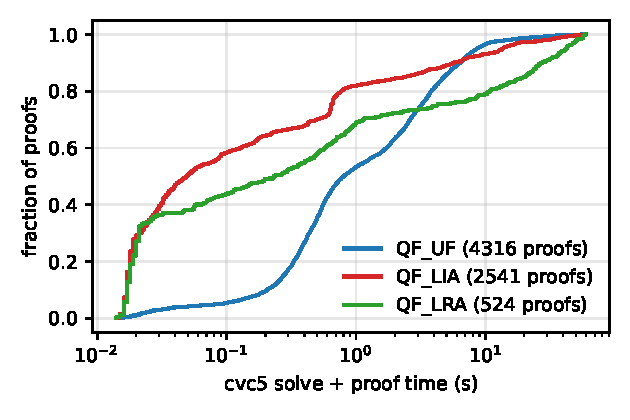
\includegraphics[width=.48\textwidth]{cvc5-time}
\caption{Left: holes per proof, as a cumulative distribution (log scale).
  Right: cvc5's solve-and-print time; every proof is complete by
  construction of the sets.}\label{fig:sizes}
\end{figure}

\begin{table}[htbp]\centering\small
\begin{tabular}{p{8.6cm}rrr}
\toprule
outcome & QF\_UF & QF\_LIA & QF\_LRA \\
\midrule
re-check \texttt{valid} & 322 & 982 & 202 \\
re-check \texttt{holey}: every hole justified, untagged holes left & 1,563 & 987 & 124 \\
re-check \texttt{holey}: every hole justified, a trust step of the elaborator left & 22 & 294 & 0 \\
re-check \texttt{holey}: a hole kept or skipped & 2,211 & 249 & 189 \\
hoist + prune rejected the proof (resolution pivot) & 198 & 2 & 6 \\
hoist + prune timeout (300 s) & 0 & 8 & 0 \\
elaboration pass external limit (1,600 s) & 0 & 16 & 3 \\
task killed at the job memory limit (60 GB) before the pass ended & 0 & 3 & 0 \\
\bottomrule
\end{tabular}

\caption{Outcome of every benchmark. The \npivot{} hoist rejections are
  cvc5 resolution steps whose pivot is not in the clause (the
  QG-classification \code{iso} family in \UF{}, two Goel, four Heizmann,
  two LassoRanker and two SMPT proofs), a cvc5 defect known from earlier
  runs. The \nhoistto{} hoist time-outs continue with the unhoisted proof:
  four of them finish the pass with holes left, four hit its external
  limit. The external limit fires when the 1,500\,s deadline expires inside
  a step the budget cannot interrupt; the passes it cut ran on proofs of
  60 to 3,900 holes, and their work is lost with the process. Three \LIA{}
  tasks (\code{SpamAssassin-loop}, \code{prp-2-17}, \code{prp-3-18}) were
  killed at the job's 60\,GB during the pass and have no record, the same
  three that were lost the same way in the earlier runs.}\label{tab:outcomes}
\end{table}

\clearpage
\section{Hole outcomes}\label{sec:passes}

Table~\ref{tab:passes} and Figure~\ref{fig:pass} give the outcome of every
hole of the proofs that ran the pass. Three numbers matter:
\begin{itemize}
  \item \textbf{Of the holes attempted}, elaboration justifies 99.5\%
    (\UF{}, \LIA{}) and 99.3\% (\LRA{}); counting the holes egglog proved
    but the reconstruction lost, the engine proves 99.96\% / 99.7\% /
    99.5\%. This is the engine's rate on cvc5's rewrite goals, and it no
    longer depends on the logic.
  \item \textbf{The budget no longer binds.} \nskipped{} holes were
    skipped in the whole run (Table~\ref{tab:budget}), against tens of
    thousands in \code{rw1}; only \LRA{} still has proofs above 10k holes,
    and they finish. Figure~\ref{fig:bysize} shows the outcome by proof
    size and Figure~\ref{fig:sizevstime} the pass time against it: the
    pass scales with the hole count and stops at the budget in a handful
    of proofs.
  \item \textbf{The normalizer does a third of the work}
    (Table~\ref{tab:normalizer}). Of the holes attempted, \normshare\%
    are closed by the normalizer alone -- both sides normalize to the same
    term under the four checker-certified procedures -- and the largest
    part of the rest goes to egglog in normal form, where it is proved at
    98--99\% and bridged back to the stated goal. The retry of the stated
    goal after the normal form fails is worth keeping on \LIA{} (2.7k of
    4.8k retries proved) and nearly worthless on \LRA{} (44 of 1.8k).
\end{itemize}

\begin{table}[htbp]\centering\footnotesize
\resizebox{\textwidth}{!}{\begin{tabular}{lrrrrrrrrr}
\toprule
logic & holes & attempted & justified & kept & skipped & \% of attempted & \% of all & proved, lost after egglog & proved, \% of all \\
\midrule
QF\_UF & 1,171,831 & 1,171,798 & 1,166,150 & 5,648 & 33 & 99.5 & 99.5 & 5,144 & 99.95 \\
QF\_LIA & 713,883 & 713,402 & 709,945 & 3,457 & 481 & 99.5 & 99.4 & 1,718 & 99.69 \\
QF\_LRA & 433,860 & 433,831 & 430,962 & 2,869 & 29 & 99.3 & 99.3 & 513 & 99.45 \\
\bottomrule
\end{tabular}
}
\caption{Hole outcomes of the pass, over the proofs that ran it.
  ``attempted'' = justified + kept; ``skipped'' = never tried because the
  budget ran out. ``proved, lost after egglog'' are the kept holes whose
  goal egglog had proved (no certificate, checker rejected, decode
  failure, or killed in the search or the serialization); the last column
  adds them to the justified ones.}\label{tab:passes}
\end{table}

\begin{figure}[htbp]\centering
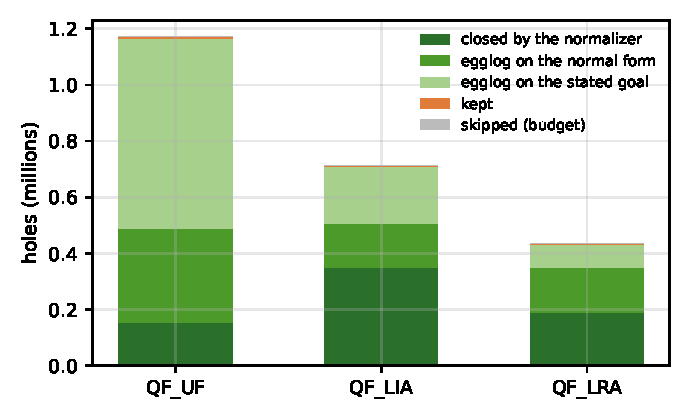
\includegraphics[width=.55\textwidth]{pass-outcome}
\caption{The same counts as a picture, with the justified holes split by
  who closed them: the normalizer alone, egglog on the normal form, or
  egglog on the stated goal.}\label{fig:pass}
\end{figure}

\begin{table}[htbp]\centering\small
\resizebox{\textwidth}{!}{\begin{tabular}{lrrrrrrr}
\toprule
logic & holes & closed by the normalizer & normal form to egglog & proved, bridged & retried as stated, proved & stated goal only & \% justified \\
\midrule
QF\_UF & 1,171,831 & 155,455 (13.3\%) & 339,484 & 333,594 & 387 of 5,890 & 676,714 & 99.5 \\
QF\_LIA & 713,883 & 349,624 (49.0\%) & 160,387 & 155,549 & 2,671 of 4,838 & 202,101 & 99.4 \\
QF\_LRA & 433,860 & 189,707 (43.7\%) & 160,464 & 158,616 & 44 of 1,848 & 82,595 & 99.3 \\
\bottomrule
\end{tabular}
}
\caption{The normalizer's share. ``closed'' are holes whose two sides
  normalize equal; ``normal form to egglog'' the holes handed to egglog as
  their normal form, of which ``proved, bridged'' came back with a
  certificate joined to the stated goal; ``retried as stated'' the ones
  whose normal form failed and whose stated goal was then tried; ``stated
  goal only'' the holes whose normal form was the goal itself.}\label{tab:normalizer}
\end{table}

\begin{table}[htbp]\centering\small
\resizebox{\textwidth}{!}{\begin{tabular}{lrrrrrr}
\toprule
logic & proofs run & hit 1,500 s & holes skipped there & hit the 1,600 s external limit & proofs $>$10k holes & \% of holes \\
\midrule
QF\_UF & 4,118 & 1 & 33 & 0 & 0 & 0.0 \\
QF\_LIA & 2,516 & 11 & 481 & 20 & 0 & 0.0 \\
QF\_LRA & 515 & 6 & 29 & 3 & 6 & 18.9 \\
\bottomrule
\end{tabular}
}
\caption{Where the pass budget binds. ``proofs run'' are the proofs with a
  pass record.}\label{tab:budget}
\end{table}

\begin{figure}[htbp]\centering
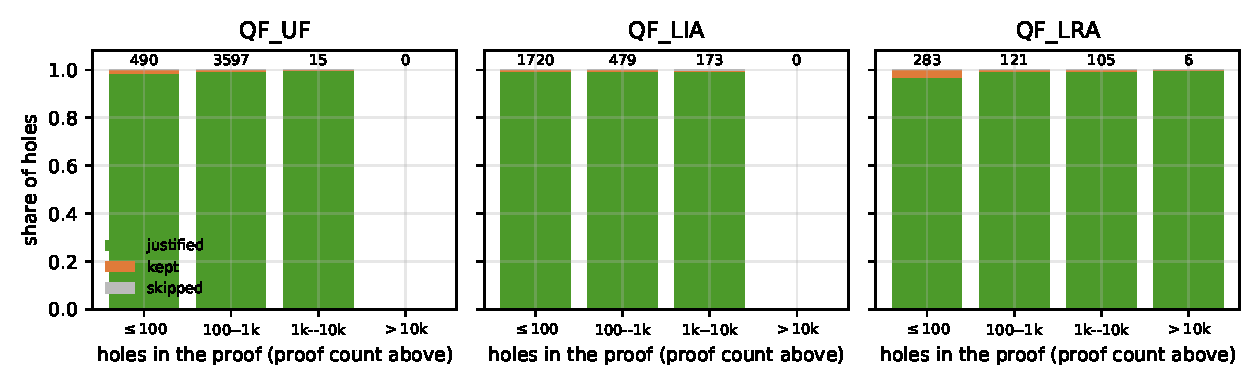
\includegraphics[width=\textwidth]{outcome-by-size}
\caption{Outcome of the holes by proof size. The budget is visible only
  in \LIA{}'s and \LRA{}'s largest bucket, and there as a sliver.}\label{fig:bysize}
\end{figure}

\begin{figure}[htbp]\centering
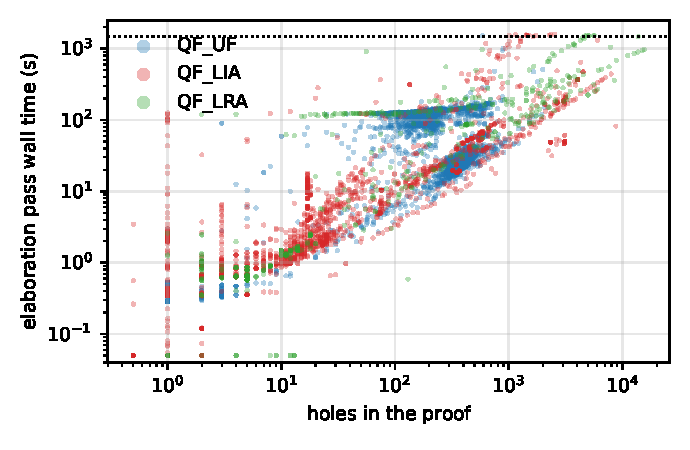
\includegraphics[width=.55\textwidth]{size-vs-time}
\caption{Pass wall time against proof size, one point per proof; the
  dotted line is the budget. The plateau at 60\,s in small proofs is a
  single hole running to its per-hole limit; the points above the budget
  are the passes the deadline could not interrupt.}\label{fig:sizevstime}
\end{figure}

\begin{table}[htbp]\centering\small
\resizebox{\textwidth}{!}{\begin{tabular}{lrrrrrr}
\toprule
logic & family & proofs & holes & \% justified & \% kept & \% skipped \\
\midrule
QF\_UF & \texttt{QG-classification} & 3,655 & 1,130,800 & 99.5 & 0.5 & 0.0 \\
QF\_UF & \texttt{2018-Goel-hwbench} & 225 & 21,632 & 98.6 & 1.3 & 0.2 \\
QF\_UF & \texttt{NEQ} & 41 & 12,970 & 100.0 & 0.0 & 0.0 \\
QF\_UF & \texttt{PEQ} & 27 & 3,828 & 100.0 & 0.0 & 0.0 \\
QF\_UF & \texttt{SEQ} & 36 & 2,260 & 100.0 & 0.0 & 0.0 \\
\midrule
QF\_LIA & \texttt{20220307-SMPT} & 1,518 & 177,392 & 99.9 & 0.1 & 0.0 \\
QF\_LIA & \texttt{mathsat} & 94 & 139,129 & 100.0 & 0.0 & 0.0 \\
QF\_LIA & \texttt{bofill-scheduling} & 245 & 116,673 & 100.0 & 0.0 & 0.0 \\
QF\_LIA & \texttt{rings} & 84 & 69,618 & 99.6 & 0.4 & 0.0 \\
QF\_LIA & \texttt{rings\_preprocessed} & 90 & 65,035 & 100.0 & 0.0 & 0.0 \\
\midrule
QF\_LRA & \texttt{uart} & 18 & 113,026 & 99.5 & 0.5 & 0.0 \\
QF\_LRA & \texttt{LassoRanker} & 65 & 95,495 & 99.9 & 0.1 & 0.0 \\
QF\_LRA & \texttt{sc} & 25 & 79,557 & 98.0 & 2.0 & 0.0 \\
QF\_LRA & \texttt{tta\_startup} & 39 & 42,439 & 99.5 & 0.5 & 0.0 \\
QF\_LRA & \texttt{clock\_synchro} & 34 & 29,096 & 99.9 & 0.1 & 0.0 \\
\bottomrule
\end{tabular}
}
\caption{The five families with the most holes per logic.}\label{tab:families}
\end{table}

\begin{figure}[htbp]\centering
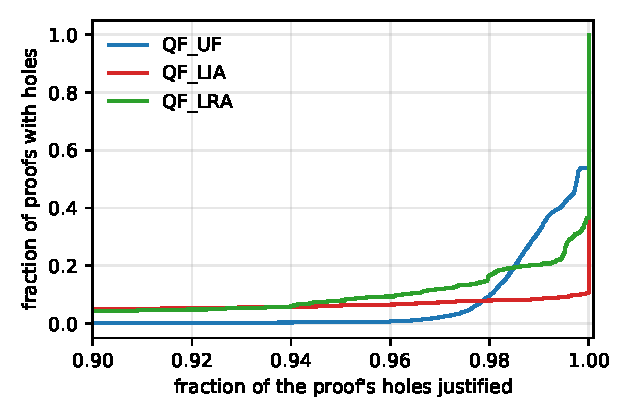
\includegraphics[width=.55\textwidth]{justified-per-proof}
\caption{Per-proof share of holes justified (the axis starts at 0.9). In
  every logic more than 90\% of the proofs have more than 99\% of their
  holes justified; the tail is Dartagnan in \LIA{} and the four
  hole-heavy families in \LRA{}.}\label{fig:perproof}
\end{figure}

\clearpage
\section{Per-hole cost}

Table~\ref{tab:timing} and Figure~\ref{fig:holetime} give the time per
hole for the holes the pass justified, once over all of them and once over
those that went through egglog (the normalizer's closures cost nothing
measurable). The \UF{} median of 0.50\,s is a floor rather than a
distribution: a worker is a child process that parses the rule file,
builds the e-graph and saturates, and the coarse Boolean holes of
QG-classification all cost the same. \LIA{}'s fat tail (115k holes over a
second) is the arithmetic saturation on whole-assertion goals.
Figure~\ref{fig:phases} and Table~\ref{tab:phases} split the time of the
holes that went through egglog into its phases: saturation is 65\% of it
on \UF{} and 82\% on the arithmetic logics, the certificate search 34\%
and 16--17\%, the snapshot under 1\%. The search's share on \UF{} is the
coarse Boolean holes again, and so are its kills: 2,875 \UF{} holes died
in the search after egglog had proved the goal, against 469 inside egglog.
Eight workers reach 3.5--5.4 cores of the 8: the parent's parsing,
hoisting and re-check are serial, and the smallest-first worklist drains
into a few long holes at the end of a proof.

\begin{table}[htbp]\centering\small
\begin{tabular}{lrrrrrrrr}
\toprule
logic & holes & finished & p50 & p90 & p99 & max & $\geq$10 s & CPU hours \\
\midrule
QF\_UF & all justified & 1,163,937 & 0.50 & 0.57 & 1.80 & 118.4 & 3,185 & 157.3 \\
 & through egglog & 1,008,678 & 0.51 & 0.58 & 1.86 & 118.4 & 3,185 & 157.3 \\
QF\_LIA & all justified & 686,232 & 0.31 & 1.26 & 4.65 & 115.3 & 3,020 & 129.7 \\
 & through egglog & 348,691 & 0.86 & 1.42 & 7.33 & 115.3 & 3,020 & 129.7 \\
QF\_LRA & all justified & 431,485 & 0.39 & 0.93 & 1.87 & 117.1 & 359 & 49.6 \\
 & through egglog & 241,581 & 0.56 & 1.11 & 2.13 & 117.1 & 359 & 49.6 \\
\bottomrule
\end{tabular}

\caption{Time per hole, holes the pass justified. The maxima above 60\,s
  are holes whose worker was killed at the limit and retried on the stated
  goal after the normal form.}\label{tab:timing}
\end{table}

\begin{figure}[htbp]\centering
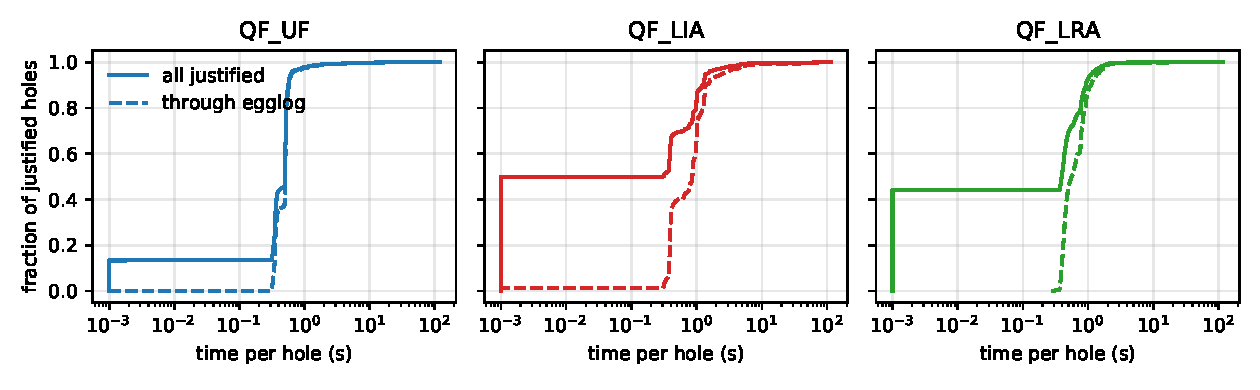
\includegraphics[width=\textwidth]{hole-time-cdf}
\caption{Per-hole time, all justified holes (solid) and those that went
  through egglog (dashed).}\label{fig:holetime}
\end{figure}

\begin{figure}[htbp]\centering
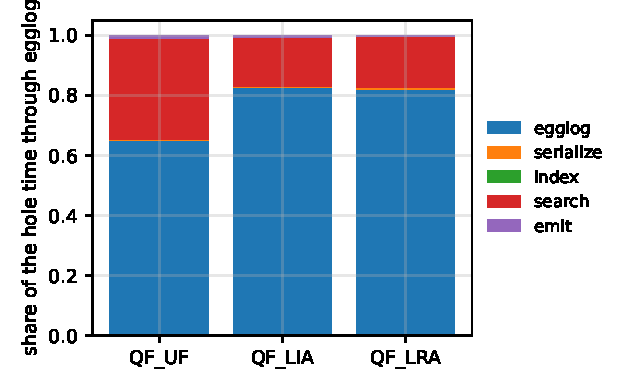
\includegraphics[width=.48\textwidth]{phases}\hfill
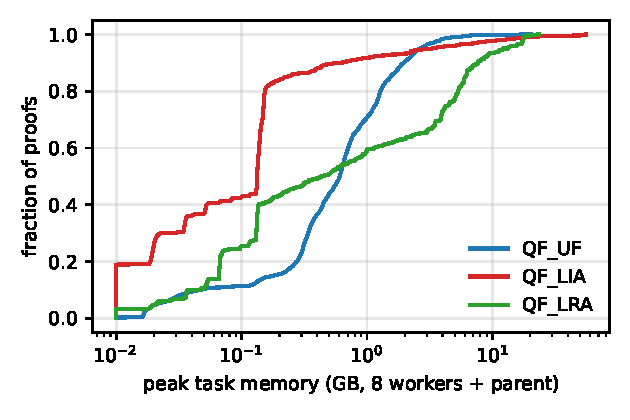
\includegraphics[width=.48\textwidth]{memory}
\caption{Left: share of the hole time per phase, holes that went through
  egglog. Right: peak memory of the task (parent plus eight workers, each
  limited to 6 GB).}\label{fig:phases}\label{fig:memory}
\end{figure}

\begin{table}[htbp]\centering\small
\begin{tabular}{lrrrrrrr}
\toprule
logic & phase & holes & p50 & p90 & max & \% of time & kills in phase \\
\midrule
QF\_UF & egglog & 1,014,214 & 0.408 & 0.425 & 60.0 & 64.9 & 469 \\
 & serialize & 1,014,214 & 0.001 & 0.002 & 2.2 & 0.4 & 2 \\
 & index & 1,014,214 & 0.000 & 0.000 & 0.3 & 0.0 & 0 \\
 & search & 1,014,214 & 0.086 & 0.134 & 59.2 & 33.7 & 2,875 \\
 & emit & 1,014,214 & 0.001 & 0.006 & 8.2 & 1.0 & 8 \\
\midrule
QF\_LIA & egglog & 359,080 & 0.746 & 1.251 & 58.5 & 82.6 & 1,254 \\
 & serialize & 359,080 & 0.002 & 0.005 & 2.1 & 0.3 & 0 \\
 & index & 359,080 & 0.000 & 0.001 & 0.4 & 0.0 & 0 \\
 & search & 359,080 & 0.094 & 0.120 & 56.3 & 16.3 & 253 \\
 & emit & 359,080 & 0.001 & 0.003 & 17.1 & 0.8 & 4 \\
\midrule
QF\_LRA & egglog & 242,412 & 0.373 & 0.970 & 55.6 & 82.1 & 2,237 \\
 & serialize & 242,412 & 0.002 & 0.004 & 4.2 & 0.4 & 0 \\
 & index & 242,412 & 0.000 & 0.001 & 0.8 & 0.0 & 0 \\
 & search & 242,412 & 0.098 & 0.141 & 51.1 & 17.1 & 26 \\
 & emit & 242,412 & 0.001 & 0.003 & 2.8 & 0.4 & 0 \\
\bottomrule
\end{tabular}

\caption{Elaboration phases per hole (seconds) and the phase a killed
  hole was in.}\label{tab:phases}
\end{table}

\clearpage
\section{Why holes are kept}\label{sec:kept}

Table~\ref{tab:reasons} and Figure~\ref{fig:reasons} classify every kept
hole by the worker's reason, and Table~\ref{tab:residue} locates them by
family. Three groups of about equal size:
\begin{itemize}
  \item \textbf{Egglog time and memory kills} (\eggshare\%). 3,814 holes hit
    the 60\,s limit inside saturation and 386 the 6\,GB limit; 2,351 of
    them are in four \LRA{} families (\code{sc}, \code{uart},
    \code{tta\_startup}, \code{spider}) and 1,000 in \LIA{}'s Dartagnan.
    They are not all size: \code{sc}'s 1,509 kills are on goals of 59 and
    114 nodes, a shape the rules blow up on (\S\ref{sec:next}).
  \item \textbf{Reconstruction losses on \UF{}'s coarse Boolean holes.}
    2,878 \UF{} holes were killed in the search after egglog had proved
    the goal, and 2,126 ended with no certificate; 137 more had their
    \code{and\_simplify} step rejected by the checker
    (Table~\ref{tab:errors}). These are the holes of QG-classification and
    Goel: Boolean simplification chains with many constant-valued
    arguments at once, which the search of \code{3f982c71} took one
    constant per congruence edge and one level per argument.
  \item \textbf{The honest residue and the checker's rejections.} 261
    goals egglog could not prove (\code{rings}, SMPT and \code{miplib}:
    a reflexive relation inside a disjunction that the normalizer closes
    but the pass had handed to egglog as stated), 177 Dartagnan
    \code{distinct\_elim} steps the checker rejected, 46 certificates the
    elaborator could not decode, and 144 holes cut by the pass budget
    mid-flight.
\end{itemize}

\begin{table}[htbp]\centering\small
\begin{tabular}{p{6.4cm}rrrr}
\toprule
reason & QF\_UF & QF\_LIA & QF\_LRA & all \\
\midrule
killed at the per-hole limit, inside egglog & 457 & 1,158 & 2,199 & 3,814 \\
killed at the per-hole limit, after egglog & 2,878 & 248 & 26 & 3,152 \\
no certificate & 2,126 & 1,242 & 486 & 3,854 \\
killed at the 6 GB limit & 27 & 245 & 114 & 386 \\
egglog could not prove & 0 & 256 & 5 & 261 \\
checker rejected & 137 & 186 & 0 & 323 \\
killed by the pass budget & 8 & 98 & 38 & 144 \\
certificate failed to decode & 3 & 42 & 1 & 46 \\
\midrule
total & 5,636 & 3,475 & 2,869 & 11,980 \\
\bottomrule
\end{tabular}

\caption{Kept holes by reason. The runner files ``egglog could not
  prove'' (an egglog \code{Check failed} verdict) and the decode failures
  under \code{worker-error}; the split here is from the messages.}\label{tab:reasons}
\end{table}

\begin{figure}[htbp]\centering
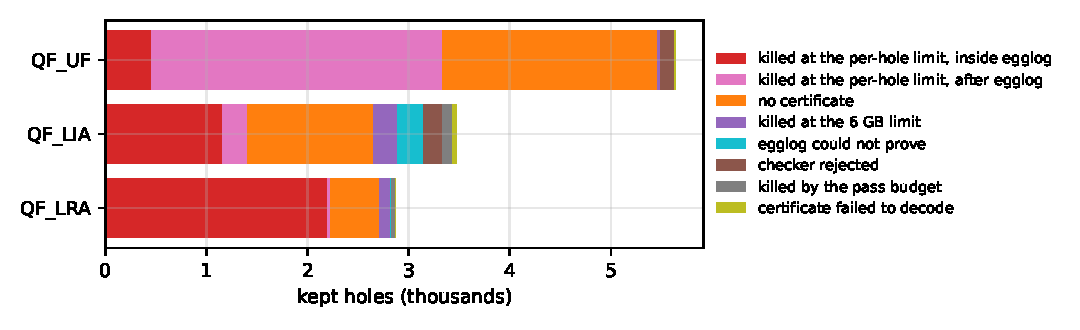
\includegraphics[width=\textwidth]{reasons}
\caption{Kept holes by reason.}\label{fig:reasons}
\end{figure}

\begin{table}[htbp]\centering\small
\begin{tabular}{lrrr}
\toprule
rule of the rejected step & QF\_UF & QF\_LIA & QF\_LRA \\
\midrule
\texttt{distinct\_elim} & 0 & 177 & 0 \\
\texttt{and\_simplify} & 138 & 0 & 0 \\
\texttt{resolution} & 0 & 6 & 0 \\
\texttt{or\_simplify} & 0 & 6 & 0 \\
\bottomrule
\end{tabular}

\caption{Reconstructed steps the checker rejected, by rule. The
  \code{and\_simplify} and \code{or\_simplify} cases found the
  complementary pair through a nested connective while the rule reads
  direct arguments only; the \code{distinct\_elim} cases are Dartagnan's.}\label{tab:errors}
\end{table}

\begin{table}[htbp]\centering\footnotesize
\resizebox{\textwidth}{!}{\begin{tabular}{llrrrrp{6.2cm}}
\toprule
logic & family & proofs & every hole justified & kept & skipped & dominant classes \\
\midrule
QF\_UF & \texttt{QG-classification} & 3,851 & 1,487 & 5,359 & 0 & 2,739 killed at the per-hole limit, after egglog, 2,103 no certificate \\
QF\_UF & \texttt{2018-Goel-hwbench} & 227 & 190 & 279 & 33 & 133 killed at the per-hole limit, after egglog, 88 killed at the per-hole limit, inside egglog \\
QF\_UF & \texttt{20190906-CLEARSY} & 11 & 5 & 8 & 0 & 6 killed at the per-hole limit, after egglog, 1 checker rejected \\
QF\_UF & \texttt{20170829-Rodin} & 20 & 18 & 2 & 0 & 2 certificate failed to decode \\
\midrule
QF\_LIA & \texttt{20210219-Dartagnan} & 78 & 2 & 2,538 & 481 & 1,063 no certificate, 787 killed at the per-hole limit, inside egglog \\
QF\_LIA & \texttt{rings} & 84 & 49 & 288 & 0 & 190 egglog could not prove, 72 killed at the per-hole limit, inside egglog \\
QF\_LIA & \texttt{2019-ezsmt} & 13 & 0 & 212 & 0 & 212 killed at the per-hole limit, inside egglog \\
QF\_LIA & \texttt{calypto} & 13 & 0 & 167 & 0 & 98 no certificate, 49 killed at the per-hole limit, inside egglog \\
QF\_LIA & \texttt{20220307-SMPT} & 1,520 & 1,407 & 120 & 0 & 11 egglog could not prove, 9 killed at the per-hole limit, inside egglog \\
QF\_LIA & \texttt{fft} & 2 & 0 & 82 & 0 & 78 no certificate, 4 killed at the per-hole limit, inside egglog \\
\midrule
QF\_LRA & \texttt{sc} & 25 & 0 & 1,597 & 29 & 1,509 killed at the per-hole limit, inside egglog, 50 no certificate \\
QF\_LRA & \texttt{uart} & 18 & 0 & 587 & 0 & 347 no certificate, 223 killed at the per-hole limit, inside egglog \\
QF\_LRA & \texttt{spider\_benchmarks} & 42 & 6 & 283 & 0 & 166 killed at the per-hole limit, inside egglog, 68 killed at the 6 GB limit \\
QF\_LRA & \texttt{tta\_startup} & 39 & 0 & 230 & 0 & 183 killed at the per-hole limit, inside egglog, 26 no certificate \\
QF\_LRA & \texttt{sal} & 96 & 61 & 79 & 0 & 52 killed at the per-hole limit, inside egglog, 20 killed at the 6 GB limit \\
QF\_LRA & \texttt{LassoRanker} & 67 & 46 & 57 & 0 & 41 killed at the per-hole limit, inside egglog, 11 no certificate \\
\bottomrule
\end{tabular}
}
\caption{The residue by family: the families with the most kept and
  skipped holes per logic.}\label{tab:residue}
\end{table}

\subsection{Reproduced and fixed after the run}\label{sec:fixed}

The smallest proof of each class of Table~\ref{tab:residue} that is not an
egglog time-out was replayed locally with the run's options (notes
\S47.11, commits \code{36cc79fa} and \code{fedf0b31}):
\begin{itemize}
  \item \textbf{Decode failures.} A congruence spine the search met from
    the far side arrives under \code{Symm} nodes, and the spine descent
    found no \code{cong} premises in it. It now reads \code{Symm} as a
    flip.
  \item \textbf{\code{and\_simplify} / \code{or\_simplify} rejections.}
    The flat form is now stated first by \code{aci\_simp}, so the checker
    sees the complementary pair as direct arguments.
  \item \textbf{No certificate on Boolean chains with many constant
    arguments.} A candidate now replaces every constant-valued subterm at
    once; the ACI computation is the checker's \code{aci\_simp} in full; a
    one-step checker computation is tried before the congruence and the
    search; and no congruence is attempted between two different heads.
  \item \textbf{A goal egglog cannot prove as stated but the normalizer
    closes.} The rule that keeps a stated goal when its normal form is
    larger is confined to the checking pass; elaboration tries the normal
    form first whatever its size, the stated goal on a failure.
\end{itemize}
Every reproducer elaborates and re-checks. The Dartagnan proof
\code{benchmark20\_conjunctive-O0} goes from 198 to 200 of 231 justified with
no rejection or decode failure left; the smallest \code{rings} proof with
unproved holes in the run justifies 349 of 349; \code{uart-5.base.cvc},
whose family had 347 no-certificate holes, keeps one of 299 (a memory kill
inside egglog). Five larger samples keep their justified counts and run
their passes in half the time (Table~\ref{tab:samples}).

\begin{table}[htbp]\centering\small
\begin{tabular}{lrr}
\toprule
proof & \code{3f982c71} (run binary) & \code{fedf0b31} \\
\midrule
\code{clocksynchro\_3clocks.main\_invar.base} & 195 of 196, 90 s & 195 of 196, 65 s \\
\code{cut\_lemma\_01\_008} & 126 of 126, 17 s & 126 of 126, 7 s \\
\code{MULTIPLIER\_3.msat} & 272 of 272, 16 s & 272 of 272, 7 s \\
\code{tgc\_io-safe-6} & 140 of 140, 12 s & 140 of 140, 5 s \\
\code{ring\_2exp10\_3vars\_1ite\_unsat} & 349 of 349, 22 s & 349 of 349, 11 s \\
\bottomrule
\end{tabular}
\caption{Five samples, holes justified and pass time, elaboration at 45\,s
  per hole on four workers.}\label{tab:samples}
\end{table}

\subsection{Limitations in the emitted proofs}\label{sec:limits}

Table~\ref{tab:valid} crosses ``every hole justified'' with the untagged
holes and the re-check. \nfullyclean{} proofs are fully justified and carry
no untagged hole, and \nfullycleanholey{} of them still re-check
\code{holey}: a certificate whose \code{arith\_poly\_norm\_rel} obligation
the relation routing cannot express through \code{poly\_simp\_rel} is
emitted as a \code{TRUST\_THEORY\_REWRITE} hole step (the \code{trusted}
fallback of \code{rare\_hole.rs}). That is 294 \LIA{} proofs, a quarter of
the \LIA{} proofs the pipeline could have closed, and the cheapest
\code{valid} gain left; the 22 \UF{} cases were not examined. The untagged
holes themselves cap \code{valid} at 2,426 / 1,393 / 204 proofs and no
Carcara change moves them.

\begin{table}[htbp]\centering\small
\resizebox{\textwidth}{!}{\begin{tabular}{lrrrrrr}
\toprule
logic & proofs with an untagged hole & every hole justified, untagged & every hole justified, no untagged & of those \texttt{valid} & of those \texttt{holey} & re-check timeouts \\
\midrule
QF\_UF & 1,890 & 1,563 & 344 & 322 & 22 & 0 \\
QF\_LIA & 1,148 & 987 & 1,276 & 982 & 294 & 21 \\
QF\_LRA & 320 & 124 & 202 & 202 & 0 & 3 \\
\bottomrule
\end{tabular}
}
\caption{Fully justified proofs against the untagged holes and the
  re-check.}\label{tab:valid}
\end{table}

\section{The tooling at \code{fedf0b31}}\label{sec:tooling}

\paragraph{Normalizer prepass} (\code{elaborator/prenorm.rs}, driven from
\code{elaborator/mod.rs}). Computes a normal form of every hole's two sides
with four checker-certified procedures: ACI normalization of \code{and} /
\code{or} (\code{aci\_simp}), polynomial normalization (\code{poly\_simp}),
relation normalization to a scaled difference with the constant on the
right (\code{poly\_simp\_rel}), and \code{distinct} elimination. It is
restricted to what core Alethe rules certify; no Boolean or equality
simplification from the \code{*\_simplify} family lives here. Integer
tightening is \emph{not} implemented, although the specification in the
notes (\S25) lists it; \S\ref{sec:next} returns to this.

\paragraph{Engine} (\code{rare/engine.rs}, \code{rare/computational/*}).
RARE rules compiled to egglog with the goal's terms as seeds; sort guard
relations keep polymorphic rules on the right sorts; a conditional rule's
premise is demanded at the occurrence of its left-hand side rather than
over all term pairs; \code{:list} parameters use the set-form encoding so
flattening, absorption and duplicate rules fire in one step; polynomial
normalization and evaluation are built-in relations; saturation runs in
bounded steps against the growth caps, the memory soft cap and the
deadline, and stops when egglog reports no update.

\paragraph{Reconstruction} (\code{rare/reconstruction/}). A certificate
search over the saturated e-graph from the goal's left class to its right
class: rule instances, congruence (one child or every constant-valued
subterm replaced at once), computations (evaluation, ACI, polynomial,
\code{distinct}), list rules on the set form, ACI-modulo matching; four
rejustifications per obligation; every certificate verified by an
independent rule checker before it is emitted.

\paragraph{Elaborator} (\code{elaborator/rare\_hole.rs}). Certificates
become Alethe steps (\code{rare\_rewrite}, \code{cong}, \code{trans},
\code{symm}, \code{refl}, \code{evaluate}, \code{aci\_simp},
\code{and\_simplify}, \code{or\_simplify}, \code{poly\_simp},
\code{poly\_simp\_rel}, \code{equiv\_simplify}, \code{ite\_simplify} and
the rest of the checker's computations), inserted at the hole with fresh
ids and re-checked in the worker before the parent accepts them. Workers
are isolated processes with a memory limit and a hard deadline; a kill is
reported with its phase and the time spent before it.

\paragraph{Tests and files.} 286 library tests, among them 13 end-to-end
elaboration fixtures in \code{tests/rare/elaborate/}, each elaborated and
re-checked \code{valid}. The static binary of \code{fedf0b31} is built and
not yet uploaded.

\section{What a rerun should change, and the three open directions}\label{sec:next}

\begin{enumerate}
  \item Rebuild the static binary from \code{fedf0b31} or later
    (\S\ref{sec:fixed}), which removes the reconstruction losses of
    \S\ref{sec:kept} on the replayed samples, and run the same three sets.
  \item Count the trust steps the elaborator emits (\S\ref{sec:limits}) in
    the runner, and extend the relation routing so that they are not
    emitted.
  \item Make the pass deadline interrupt the non-hole checking (23
    external kills), and raise the re-check limit for the largest
    elaborated proofs (\nrecheckto{} time-outs at 900\,s).
\end{enumerate}

\paragraph{Dartagnan's arithmetic Boolean chains (\LIA{}).} 78 proofs, 2
fully justified, 3,019 holes lost; after the fixes,
\code{benchmark20\_conjunctive-O0} still keeps 31 of 231 (22 no certificate, 4
memory, 2 time). The goals are cvc5's rewrite of a whole assertion: an
implication whose antecedent is a conjunction of bound pairs
\code{(and (<= a b) (>= a b))} and equalities \code{(= x 1)}, rewritten into
a flat conjunction of \code{(not (>= ...))} / \code{(>= ... 1)} literals (the
integer tightening of \code{<} and \code{>}), with \code{ite}-valued terms
in the polynomials, 50--800 nodes; one 16-node case,
\code{(= (ite c true true) true) = true}, has no certificate either, so at
least one gap is a plain search gap. Plan: (1) micro-reproducers from the
22 goals, the \code{ite} case first (egglog proves it, so the search does
not see the \code{ite-eq-branch} instance or discards the congruence into
the \code{true} class); (2) a structural descent before the search -- when
both sides share the head, prove the children pairwise and join with
\code{cong}, so that a whole-assertion goal becomes its 10--80 independent
atom goals, each of which the search already proves; (3) a rejustification
budget set from the goal's atom count, if the debug trace of the 22 goals
says four is the cap that bites; (4) for the egglog time and memory kills,
the per-ruleset run report on the smallest such goal, the polynomial rules
on \code{ite} arguments being the first suspect; (5) a local batch of all
78 proofs (cvc5 solves each in under a second) as the exit criterion,
70 of 78 fully justified and no no-certificate class left, then the
cluster run.

\paragraph{The hole-heavy \LRA{} families.} \code{sc}, \code{uart},
\code{tta\_startup}, \code{spider}, \code{sal}, \code{LassoRanker},
\code{clock\_synchro}: 2,852 holes lost, 2,351 of them egglog time or
memory kills, and two different problems behind them. Small goals the
rules blow up on: \code{sc}'s 1,509 kills are on goals of 59 and 114
nodes, and \code{sc-5.base.cvc} replayed locally (415 holes) keeps 14 --
7 goals of 59 nodes that fail \emph{fast} (no rule path), 5 of 114 nodes
that saturate for 60\,s, 2 without certificate -- all
\code{MACRO\_SR\_PRED\_INTRO} disjunctions of transition conjunctions in
which cvc5 flattened the \code{and}s, oriented the equalities, turned
\code{<=} atoms into \code{(>= (+ ...) 0.0)} mirrors and pushed \code{ite}s
into the polynomials; \code{uart}'s memory kill (\code{t262}, 179 nodes) is
the same family one size down from its 333-node time-outs. And size:
\code{tta\_startup} (900--11,000 nodes), \code{LassoRanker} (3,000--8,700),
\code{clock\_synchro} (2,000--3,400) and \code{spider}'s 510-node memory
kills, where saturation over the whole assertion does not finish. Plan:
(1) the 59-node \code{sc} goal split into its disjuncts and conjuncts to
find the pair egglog cannot join (candidates: the \code{<=} to \code{>=}
mirror over a negated difference, which the normalizer does not orient and
\code{comp\_simplify} would certify; an equality against a normalized
polynomial; \code{(= x (ite c a b))} lifting); (2) the 114-node goal
profiled per ruleset with the \code{ite}-abstracted goal as control, and
\code{ite} excluded from the polynomial relation's argument positions if
that is the cause, as the normalizer already does; (3) the structural
descent above for the big goals, each atom pair normalized first and only
the differing pairs sent to egglog as their own small worker calls, plus a
per-hole limit scaled by goal size; (4) the smallest proof of each of the
seven families fully justified locally as the exit criterion, then the
cluster run.

\paragraph{Integer infeasibility.} The goal is
\code{(= (+ (* 3 x1) (* 3 x2)) 1) = false} (\LIA{} \code{check},
\code{int\_incompleteness1}; two holes in the run).
Egglog has no rule path, since \code{arith-int-eq-conflict} needs the
\code{(= (to\_real t) c)} shape; the normalizer scales the relation by the
reciprocal of the coefficients' gcd, producing \code{(= (+ x1 x2) 1/3)},
and stops, because the integer tightening its specification lists is not
implemented. A hand-written proof of the closed form checks \code{valid}
with the current checker: two \code{la\_generic} steps, one per direction
(\code{(cl (not (= s 1)) (>= (+ x1 x2) 1))} with coefficients $1/3$ and
$1$, and its mirror with $-1/3$ and $1$; the negation of the bound is
strengthened by \code{la\_generic}'s integer gcd rule), their resolution,
and \code{equiv\_simplify} with \code{equiv2} to state the equality. Plan:
(1) implement the tightening in the normalizer's \code{relation\_step}
(a relation whose scaled bound is non-integral is decided or rounded,
certified by the \code{la\_generic} pair -- a core rule, so within the
normalizer's remit), which also gives it the \code{(> t 0)} to
\code{(>= t 1)} step cvc5 applies throughout Dartagnan and SMPT; (2)
alternatively, present an Int relation with a Real constant to the engine
in the \code{to\_real} shape so that the RARE tightening rules fire; (3) a
fixture from \code{int\_incompleteness1}'s hole; (4) both \code{check}
benchmarks fully justified, and the count of \code{arith-geq-tighten}
certificates in the Dartagnan and SMPT replays before and after.

\appendix
\section{Files}
\begin{itemize}
  \item Results: \code{\textasciitilde/exp/results/egglog-holes/rw2/results.json.gz}
    (JSONL; one record per benchmark with the runner's full output).
  \item Analysis: \code{report-rw2/make-rw2.py} in the worktree, which
    produced every table and figure here;
    \code{\textasciitilde/exp/egglog-holes/analysis-rw2/} holds the readers
    behind the notes.
  \item Runner and submission: \code{\textasciitilde/exp/egglog-holes/run-holes-rw2.sh},
    \code{submit-egglog-rw2.sh}, \code{gen-rw-sets.py}.
  \item Notes: \code{EGGLOG-ELABORATION-NOTES.md} \S47.9--47.13 in the
    Carcara worktree; the replays of \S\ref{sec:fixed} and
    \S\ref{sec:next} are in the session scratchpad
    (\code{rw1/werr}, \code{rw1/lra}, \code{gcd}).
\end{itemize}
\end{document}
